\section{TSTL Tools}

The following tools are provided in the TSTL distribution on github \cite{tstl}.  Installing the TSTL module allows the compiler, called {\tt tstl} to be used at the command line.  Other tools are included in the {\tt generators} and {\tt utilities} directories of the distrbution as Python scripts.

\subsection{The TSTL Compiler}

Given a harness file defined in the language discussed above, the TSTL compiler generates a stand-alone Python class that allows testing of the SUT.  This generated code does not depend on the TSTL system being installed, only on any modules the testing itself uses, and on whether code coverage is requested.  By default, the compiler produces a class supporting code coverage using the {\tt coverage.py} module, and assumes this is installed.  The TSTL compiler also allows a user to control some fine-grained coverage measures, and force a system where state-storage based backtracking is impossible to use test-replay based backtracking.

\subsection{Generators}

TSTL comes with a complex, highly configurable, pure random tester (supporting numerous command-line options), and simple depth-first-search and breadth-first-search based backtracking model checkers.  The included random tester provides a number of useful options:

\begin{itemize}
\item Log all testing activity as it takes place, so that even if a test crashes Python it can be replayed, reduced, and converted into a standalone test.
\item Produce on-the-fly, time-stamped code coverage information, for analyzing performance of testing algorithms.
\item Produce ``quick test'' files \cite{icst14}, each containing a minimal path to cover a set of branches of the SUT.
\item Apply additional, custom term-rewriting based simplifications of test cases that often further minimize delta-debugged test cases; apply generalization that elaborates each failing test with annotations of similar tests that also fail.
\end{itemize}

\subsection{Visualization of Action Spaces}

\begin{figure}
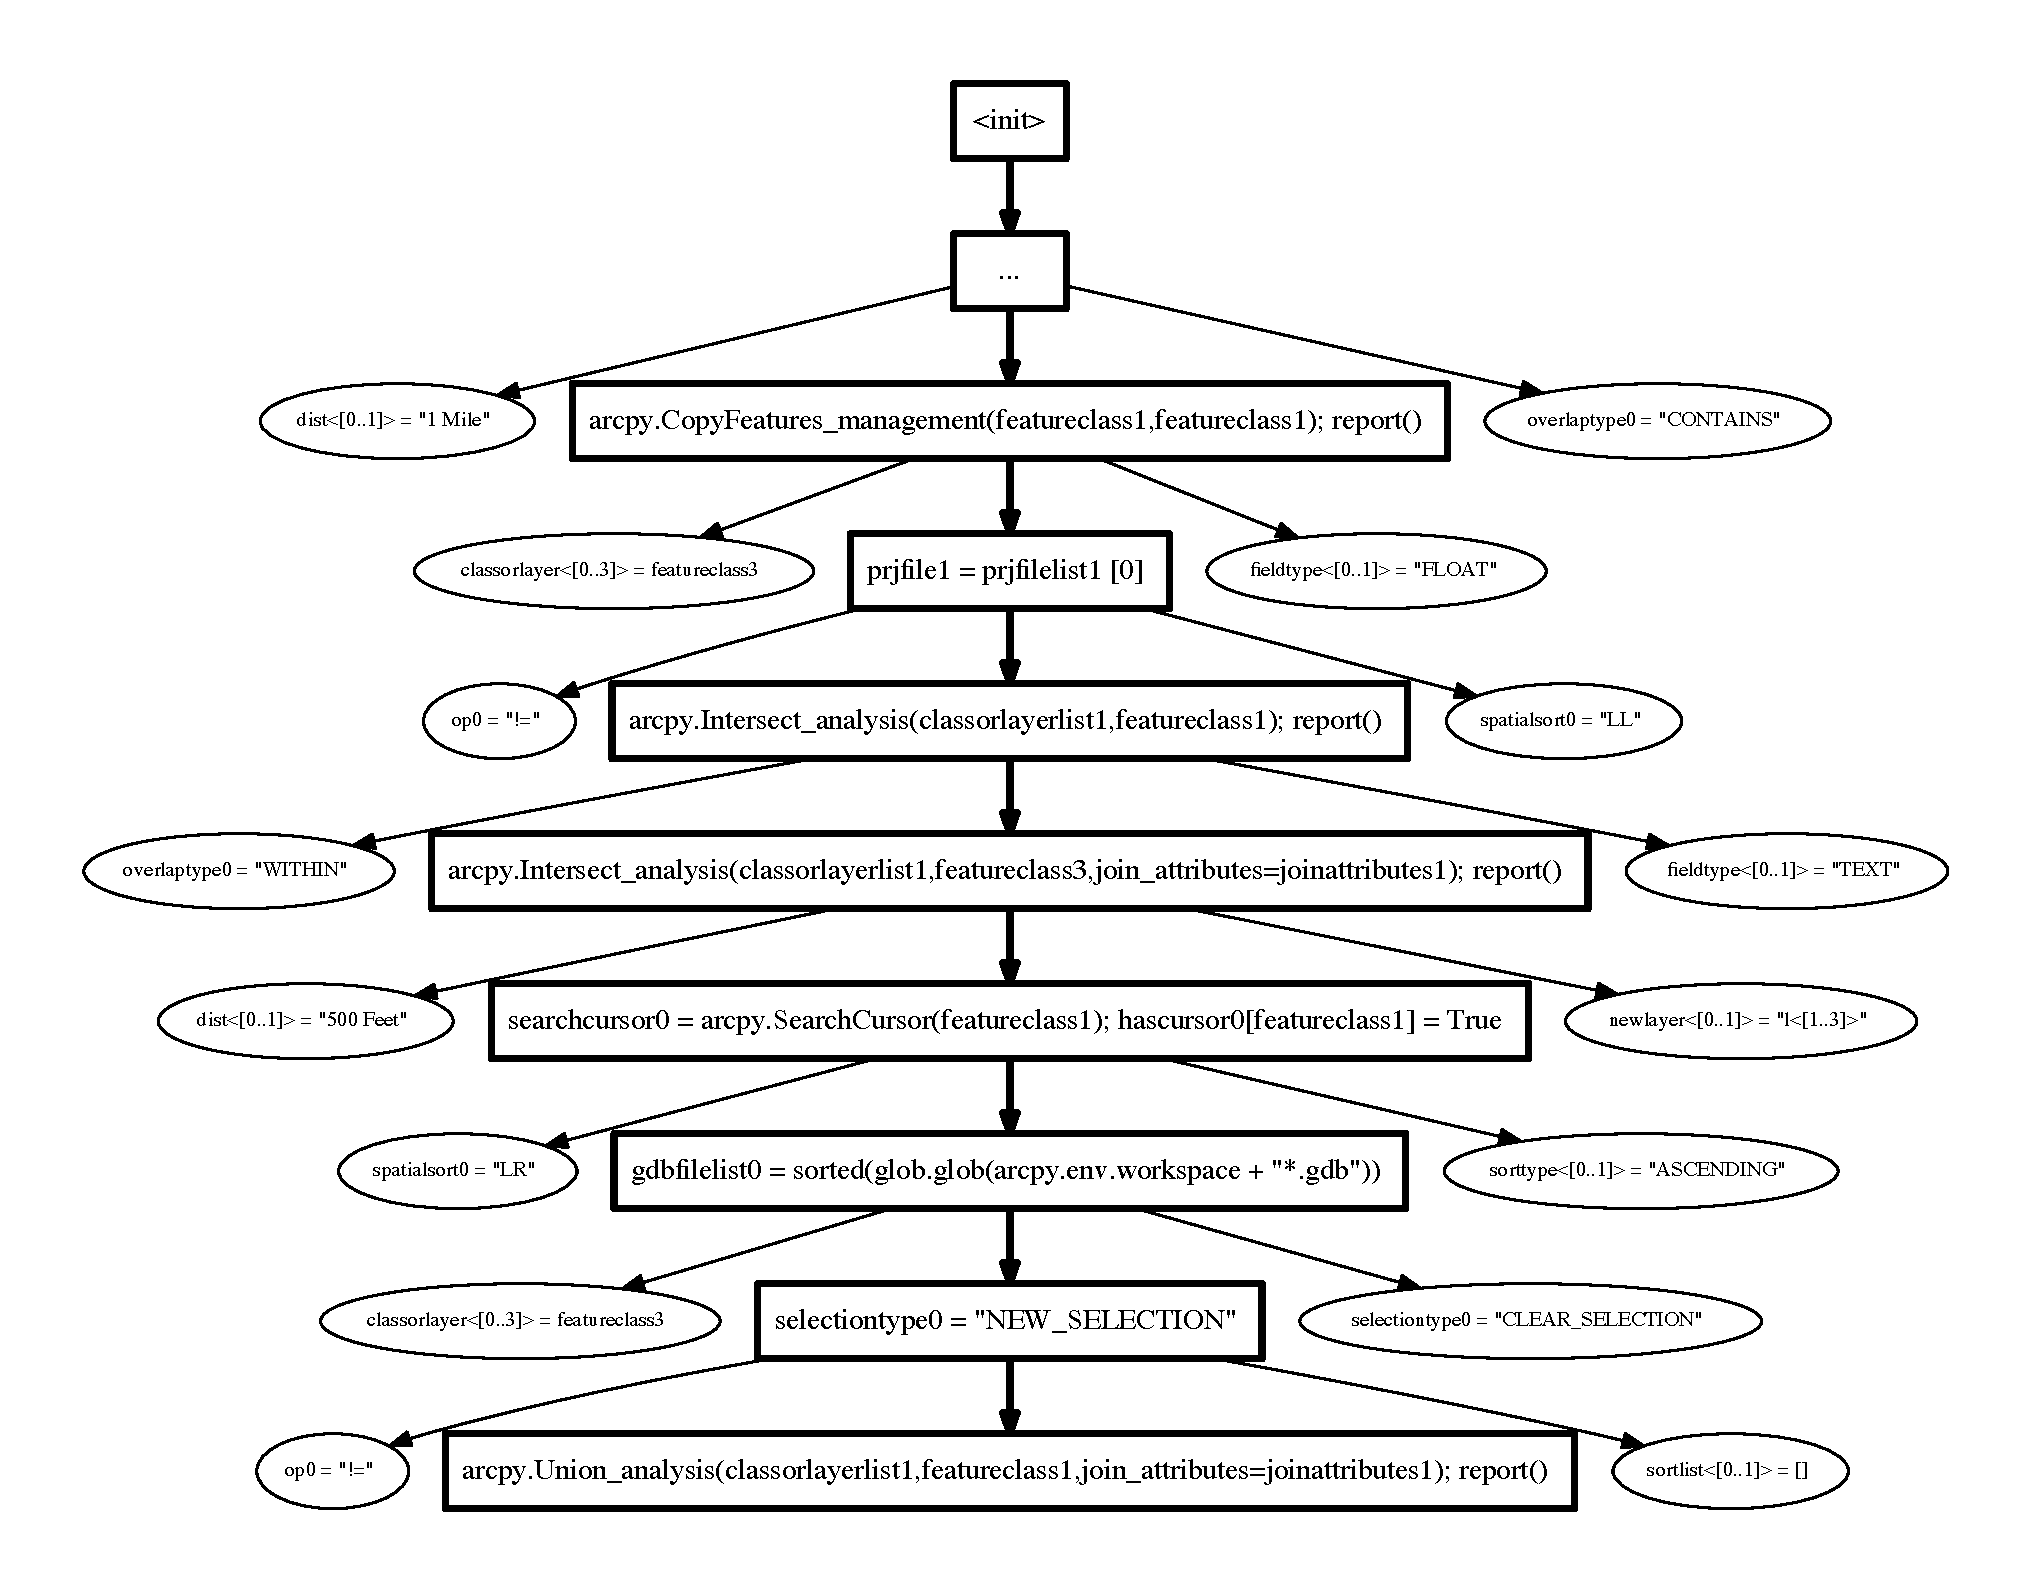
\includegraphics[width=\columnwidth]{shortgraph}
\caption{Start depth 20, depth 11, width 3 trace visualization for ArcPy testing.}
\label{fig:actions}
\end{figure}

Understanding the structure of the action graph produced by even a relatively simple TSTL harness can be difficult.  The structure is often infinite, and even in cases where there is a finite state space (perhaps introduced by abstraction) the graph is usually far too large for a convenient display.  However, we have found that a visual representation of typical trajectories through the system can be very helpful for understanding a complex test system.  The {\tt makegraph} utility takes as input a number of traces to produce, a starting depth, additional depth, and a test width.  It then produces in pdf form a number of graphs for traces like the one shown in Figure \ref{fig:actions}.  These trace graphs show, in bold, the actual action sequence chosen by a pure random tester, starting after a number of actions not shown (represented by the ``...'' node) and continuing up to the depth limit.  In addition to the actions taken, the graph also shows a random subset of additional enabled actions, with each step showing a number of actions equal to the width.  Because many actions are extremely similar, the graphing utility also summarizes actions that are the same, except for pool choice or integer constant, using the {\tt <[i..j]>} notation of TSTL.

\section{Building Your Own Tools}

Describing the full interface provided by TSTL for use in testing tools is beyond the scope of this paper.  However, examining the source code of the included testers can provide a good starting point.  Implementing new test case manipulations usually involves understanding TSTL internal structures and how tests are stored.  However, implementing novel test generation algorithms can often rely on just a handful of methods, shown in Figure \ref{methods}.

\begin{figure}
{\scriptsize
\begin{itemize}
\item {\bf restart():}  resets the system state and aborts the current test. 
\item {\bf enabled():} returns a list of all currently enabled actions.
\item {\bf randomEnabled(random):}  given a Python random number generator object, returns a random enabled action, efficiently.
\item {\bf safely(action):} performs action (usually changing SUT state)  and returns a Boolean indicating whether the action performed raised any uncaught exceptions. 
\item {\bf check():} returns a Boolean indicating whether the action performed raised any uncaught exceptions.
\item {\bf error():} returns either {\tt None} (no error for the last action or {\tt check}), or a Python object representing an uncaught exception or failed property's backtrace.
\item {\bf state():} returns the current SUT state, as a set of values for all pools; for systems where state cannot be restored by pool values, or {\tt deepcopy} does not work, returns the current test to replay (can be controlled at runtime, or set as default for an SUT).
\item {\bf backtrack(state):} takes a state produced by {\tt state} and restores the system to that state; replays a test, if state-based backtracking is turned off.
\end{itemize} 
}
\caption{Core methods for testing an SUT.}
\label{methods}
\end{figure}